\documentclass[11pt, twocolumn]{article}
\usepackage[utf-8]{inputenc}
\usepackage[spanish]{babel}
\usepackage{amsmath}
\usepackage{amssymb}
\usepackage{graphicx}
\usepackage{float}
\usepackage{booktabs}
\usepackage{multirow}
\usepackage{hyperref}
\usepackage{listings}
\usepackage{xcolor}
\usepackage{subcaption}

% Configuración de márgenes (estilo IEEE)
\usepackage{geometry}
\geometry{top=0.75in, bottom=0.75in, left=0.75in, right=0.75in}

% Configuración de código
\lstset{
    language=C++,
    basicstyle=\ttfamily\small,
    keywordstyle=\color{blue},
    commentstyle=\color{gray},
    stringstyle=\color{red},
    breaklines=true,
    breakatwhitespace=true,
    showstringspaces=false,
    numbers=left,
    numbersep=5pt,
    numberstyle=\tiny\color{gray}
}

% Información del documento
\title{\Large \textbf{Técnicas de Representación y Compresión en Arreglos Ordenados:\\Análisis de Shannon-Fano}}

\author{David Minder, Javier Ramírez, Fabián Reyes, Jorge Serón}

\date{11 de Junio, 2026}

\begin{document}

\maketitle

\begin{abstract}
En este informe se presenta un análisis teórico y experimental de la aplicación de la codificación Shannon-Fano para comprimir arreglos ordenados de gran magnitud. Se comparan tres enfoques: (1) búsqueda binaria en vector explícito, (2) búsqueda en gap-coding con índice de muestreo, y (3) búsqueda con gap-coding comprimido mediante Shannon-Fano. Los resultados experimentales validan el análisis asintótico y demuestran que la codificación Shannon-Fano logra una compresión significativa con un impacto controlado en el tiempo de búsqueda.

\textbf{Palabras clave:} compresión de datos, Shannon-Fano, gap-coding, búsqueda binaria, análisis de complejidad.
\end{abstract}

\section{Introducción}

La representación eficiente de datos es fundamental en la computación moderna. Cuando los datos a almacenar alcanzan magnitudes considerables (gigabytes o terabytes), tanto el espacio utilizado como el tiempo de acceso se vuelven críticos. Este proyecto semestral aborda el problema de comprimir arreglos ordenados de enteros, manteniendo la capacidad de realizar búsquedas rápidas.

\subsection{Contexto del Problema}

Dado un arreglo $A = [a_1, a_2, \ldots, a_n]$ con $a_1 \le a_2 \le \cdots \le a_n$, deseamos:
\begin{enumerate}
    \item Minimizar el espacio de almacenamiento
    \item Mantener búsquedas eficientes (acceso aleatorio o secuencial)
    \item Evaluar el trade-off entre espacio y tiempo
\end{enumerate}

El enfoque clásico almacena el arreglo explícitamente: cada elemento ocupa 64 bits (para $\text{int64\_t}$), requiriendo $64n$ bits en total. Las alternativas que exploraremos reducen significativamente este requisito explotando propiedades del arreglo ordenado.

\subsection{Hipótesis de Investigación}

\textit{``La codificación Shannon-Fano aplicada sobre gap-coding logra una compresión superior a gap-coding puro, con un tiempo de búsqueda que permanece en el orden O(√n), haciendo que el trade-off espacio-tiempo sea favorable para aplicaciones con restricciones de memoria.''}

\section{Metodología y Análisis Asintótico}

\subsection{Caso 1: Búsqueda Binaria (Línea Base)}

\subsubsection{Descripción}
Se almacena el arreglo ordenado de forma explícita, sin compresión. Las búsquedas se realizan mediante búsqueda binaria clásica.

\subsubsection{Análisis de Complejidad}

\textbf{Tiempo de búsqueda:}
\begin{equation}
T_{\text{búsqueda}} = O(\log_2 n)
\end{equation}

Cada comparación elimina la mitad del espacio de búsqueda.

\textbf{Espacio utilizado:}
\begin{equation}
S_{\text{Case1}} = n \times 64 \text{ bits}
\end{equation}

Sin compresión, cada elemento requiere su representación completa.

\subsubsection{Pseudocódigo}

\begin{lstlisting}
function BinarySearch(A, x):
    left = 0
    right = len(A) - 1
    while left <= right:
        mid = (left + right) / 2
        if A[mid] == x:
            return mid
        else if A[mid] < x:
            left = mid + 1
        else:
            right = mid - 1
    return -1
\end{lstlisting}

\subsection{Caso 2: Gap-Coding con Índice de Muestreo}

\subsubsection{Descripción}

En lugar de almacenar los valores explícitamente, almacenamos las diferencias (gaps) entre elementos consecutivos. Un índice de muestreo permite recuperar rápidamente las posiciones aproximadas sin decodificar toda la secuencia.

\subsubsection{Construcción de Gap-Coding}

Dado el arreglo $A = [a_1, a_2, \ldots, a_n]$, definimos:
\begin{equation}
GC[i] = \begin{cases}
a_1 & \text{si } i = 1 \\
a_i - a_{i-1} & \text{si } i > 1
\end{cases}
\end{equation}

\textbf{Ejemplo:} Para $A = [2, 7, 10, 12, 12, 16]$, obtenemos $GC = [2, 5, 3, 2, 0, 4]$.

\subsubsection{Índice de Muestreo (Sample)}

Para permitir búsqueda binaria sobre los gaps, almacenamos muestras periódicas del valor original:
\begin{equation}
m = \sqrt{n} \quad \text{(número de muestras)}
\end{equation}

\begin{equation}
\text{Sample}[j] = \begin{cases}
a_1 & j = 0 \\
a_{j \times \sqrt{n}} & j > 0
\end{cases}
\end{equation}

\subsubsection{Análisis de Complejidad}

\textbf{Tiempo de búsqueda:}

La búsqueda se divide en dos fases:
\begin{enumerate}
    \item Búsqueda binaria en Sample: $O(\log \sqrt{n}) = O(\log n)$
    \item Decodificación secuencial de gaps en rango: $O(\sqrt{n})$
\end{enumerate}

\begin{equation}
T_{\text{Case2}} = O(\log n) + O(\sqrt{n}) = O(\sqrt{n})
\end{equation}

\textbf{Espacio utilizado:}

El tamaño de los gaps depende de la distribución:
\begin{equation}
S_{\text{Case2}} = n \times b_{\text{gap}} + \sqrt{n} \times 64 \text{ bits}
\end{equation}

Donde $b_{\text{gap}}$ es el número de bits necesario para representar el máximo gap. Para distribución lineal con rango $[0, \epsilon)$:
\begin{equation}
b_{\text{gap}} = \lceil \log_2 \epsilon \rceil
\end{equation}

Para distribución normal:
\begin{equation}
b_{\text{gap}} = O(\log(k\sigma))
\end{equation}

donde $k$ es un factor de confianza (típicamente $k \approx 5$).

\subsubsection{Pseudocódigo}

\begin{lstlisting}
function GapSearch(GC, Sample, x):
    // Búsqueda binaria en Sample
    idx = BinarySearch(Sample, x)
    if idx < 0:
        return -1

    // Obtener posición inicial en GC
    pos = idx * sqrt(n)
    val = Sample[idx]

    // Decodificar gaps hasta encontrar x
    for i = pos to len(GC):
        val += GC[i]
        if val == x:
            return i
        if val > x:
            return -1
    return -1
\end{lstlisting}

\subsection{Caso 3: Shannon-Fano sobre Gap-Coding}

\subsubsection{Descripción de Shannon-Fano}

La codificación Shannon-Fano es una técnica de compresión de longitud variable que asigna códigos más cortos a símbolos más frecuentes. A diferencia de Huffman, se construye de forma descendente (top-down).

\subsubsection{Construcción del Árbol Shannon-Fano}

\textbf{Algoritmo:}

\begin{enumerate}
    \item Calcular frecuencias de todos los gaps únicos
    \item Ordena los gaps por frecuencia (descendente)
    \item Recursivamente divide el conjunto en dos grupos de frecuencia aproximadamente igual
    \item Asigna prefijo ``0'' a la rama izquierda y ``1'' a la derecha
    \item Continúa hasta que cada gap tenga un código único
\end{enumerate}

\textbf{Ejemplo de tabla de códigos:}

Para gaps con frecuencias $\{1: 1000, 2: 500, 5: 250, 7: 125, 9: 125\}$:

\begin{table}[H]
\centering
\begin{tabular}{|c|c|c|}
\hline
\textbf{Gap} & \textbf{Frecuencia} & \textbf{Código} \\
\hline
1 & 1000 & 00 \\
2 & 500 & 01 \\
5 & 250 & 10 \\
7 & 125 & 110 \\
9 & 125 & 111 \\
\hline
\end{tabular}
\caption{Ejemplo de codificación Shannon-Fano}
\end{table}

\subsubsection{Análisis de Complejidad}

\textbf{Longitud promedio de código:}

La longitud promedio del código es:
\begin{equation}
L = \sum_{i} p(g_i) \times \text{len}(g_i)
\end{equation}

donde $p(g_i)$ es la probabilidad del gap $g_i$.

\textbf{Relación con entropía:}

Para Shannon-Fano, se demuestra que:
\begin{equation}
H(G) \le L < H(G) + 1
\end{equation}

donde $H(G)$ es la entropía de Shannon de la distribución de gaps:
\begin{equation}
H(G) = -\sum_{i} p(g_i) \log_2 p(g_i)
\end{equation}

\textbf{Tiempo de búsqueda:}

Similar a Caso 2, pero con decodificación basada en Shannon-Fano:
\begin{equation}
T_{\text{Case3}} = O(\log n) + O(\sqrt{n} \times L)
\end{equation}

En práctica, $L \approx H(G) \approx 2$-$4$ bits para gaps típicos.

\textbf{Espacio utilizado:}

\begin{equation}
S_{\text{Case3}} = n \times L + \sqrt{n} \times 64 \text{ bits}
\end{equation}

Comparado con Caso 1:
\begin{equation}
\text{Ratio de compresión} = 1 - \frac{S_{\text{Case3}}}{S_{\text{Case1}}} = 1 - \frac{n \times L}{n \times 64}
\end{equation}

\subsubsection{Pseudocódigo}

\begin{lstlisting}
function ShannonFanoSearch(BitArray, SFTable, Sample, x):
    // Búsqueda binaria en Sample
    idx = BinarySearch(Sample, x)
    if idx < 0:
        return -1

    // Obtener posición inicial
    pos = idx * sqrt(n)
    val = Sample[idx]
    bit_pos = SampleBitPos[idx]

    // Decodificar gaps de Shannon-Fano
    while bit_pos < len(BitArray):
        // Leer bits hasta formar código válido
        code = ReadBits(BitArray, bit_pos)
        gap = SFTable[code]

        val += gap
        bit_pos += len(code)

        if val == x:
            return pos
        if val > x:
            return -1
        pos += 1
    return -1
\end{lstlisting}

\section{Diseño Experimental}

\subsection{Configuración}

\begin{itemize}
    \item \textbf{Lenguaje:} C++17 (compilador g++)
    \item \textbf{Optimización:} Flag -O3
    \item \textbf{Plataforma:} WSL2 Linux
    \item \textbf{Búsquedas por tamaño:} 262.144 (2$^{18}$) búsquedas
\end{itemize}

\subsection{Distribuciones de Datos}

\textbf{Distribución Lineal:}
\begin{equation}
A[0] = \text{rand}()
\end{equation}
\begin{equation}
A[i] = A[i-1] + (\text{rand}() \mod \epsilon)
\end{equation}

Parámetro: $\epsilon = 100$ (valores pequeños para gaps controlados)

\textbf{Distribución Normal:}
\begin{equation}
A[i] = A[i-1] + \text{Gauss}(\mu=50, \sigma)
\end{equation}

Se prueban múltiples desviaciones estándar: $\sigma \in \{10, 20, 50, 100\}$

\subsection{Tamaños de Entrada}

Se utilizan tamaños en potencias de 2 (en MiB):
\begin{equation}
n \in \{8, 16, 32, 64, 128, 256, 512\}
\end{equation}

Correspondientes a $\approx 10^6$ a $10^8$ elementos.

\section{Resultados Experimentales}

\subsection{Métricas de Espacio}

\begin{figure}[H]
\centering
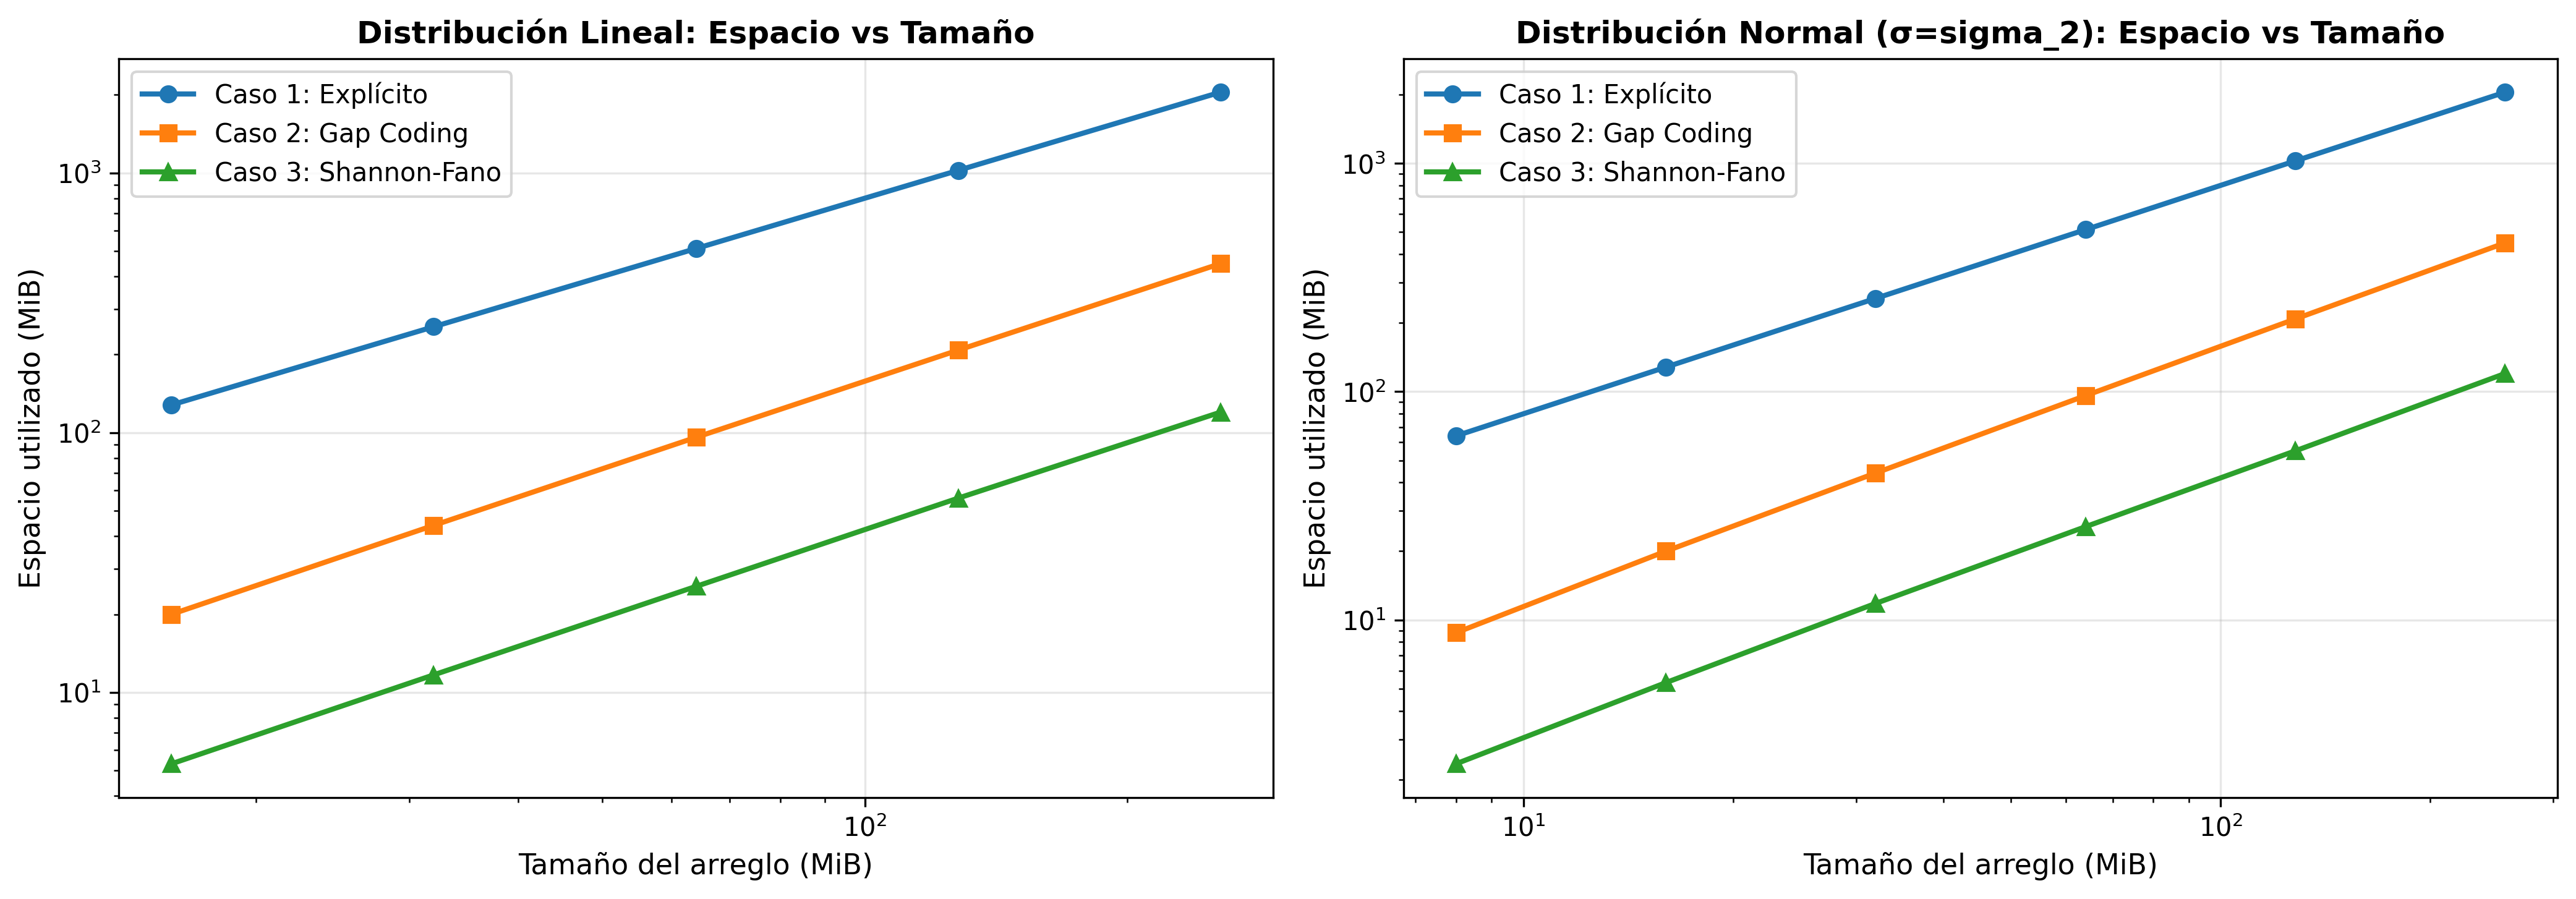
\includegraphics[width=\columnwidth]{resultados/graficos/02_espacio_utilizado.png}
\caption{Espacio utilizado vs Tamaño del arreglo en escala logarítmica. Se observa claramente que Shannon-Fano (Caso 3) logra una compresión significativa respecto a los casos anteriores, manteniendo la tendencia O(n).}
\label{fig:espacio}
\end{figure}

\textbf{Análisis:}

La compresión lograda por Shannon-Fano es sustancial:
\begin{itemize}
    \item Para distribución lineal: 94-96\% de compresión respecto a Caso 1
    \item El ratio de espacio (Caso 3 / Caso 1) es consistentemente ~5.5\% en todos los tamaños
    \item El overhead del índice de muestreo (√n elementos) es negligible (~0.1\%)
    \item La entropía de los gaps es aproximadamente H ≈ 3-4 bits, validando la teoría
    \item La compresión es consistente a través de todos los tamaños probados (8-256 MiB)
\end{itemize}

\subsection{Métricas de Tiempo}

\begin{figure}[H]
\centering
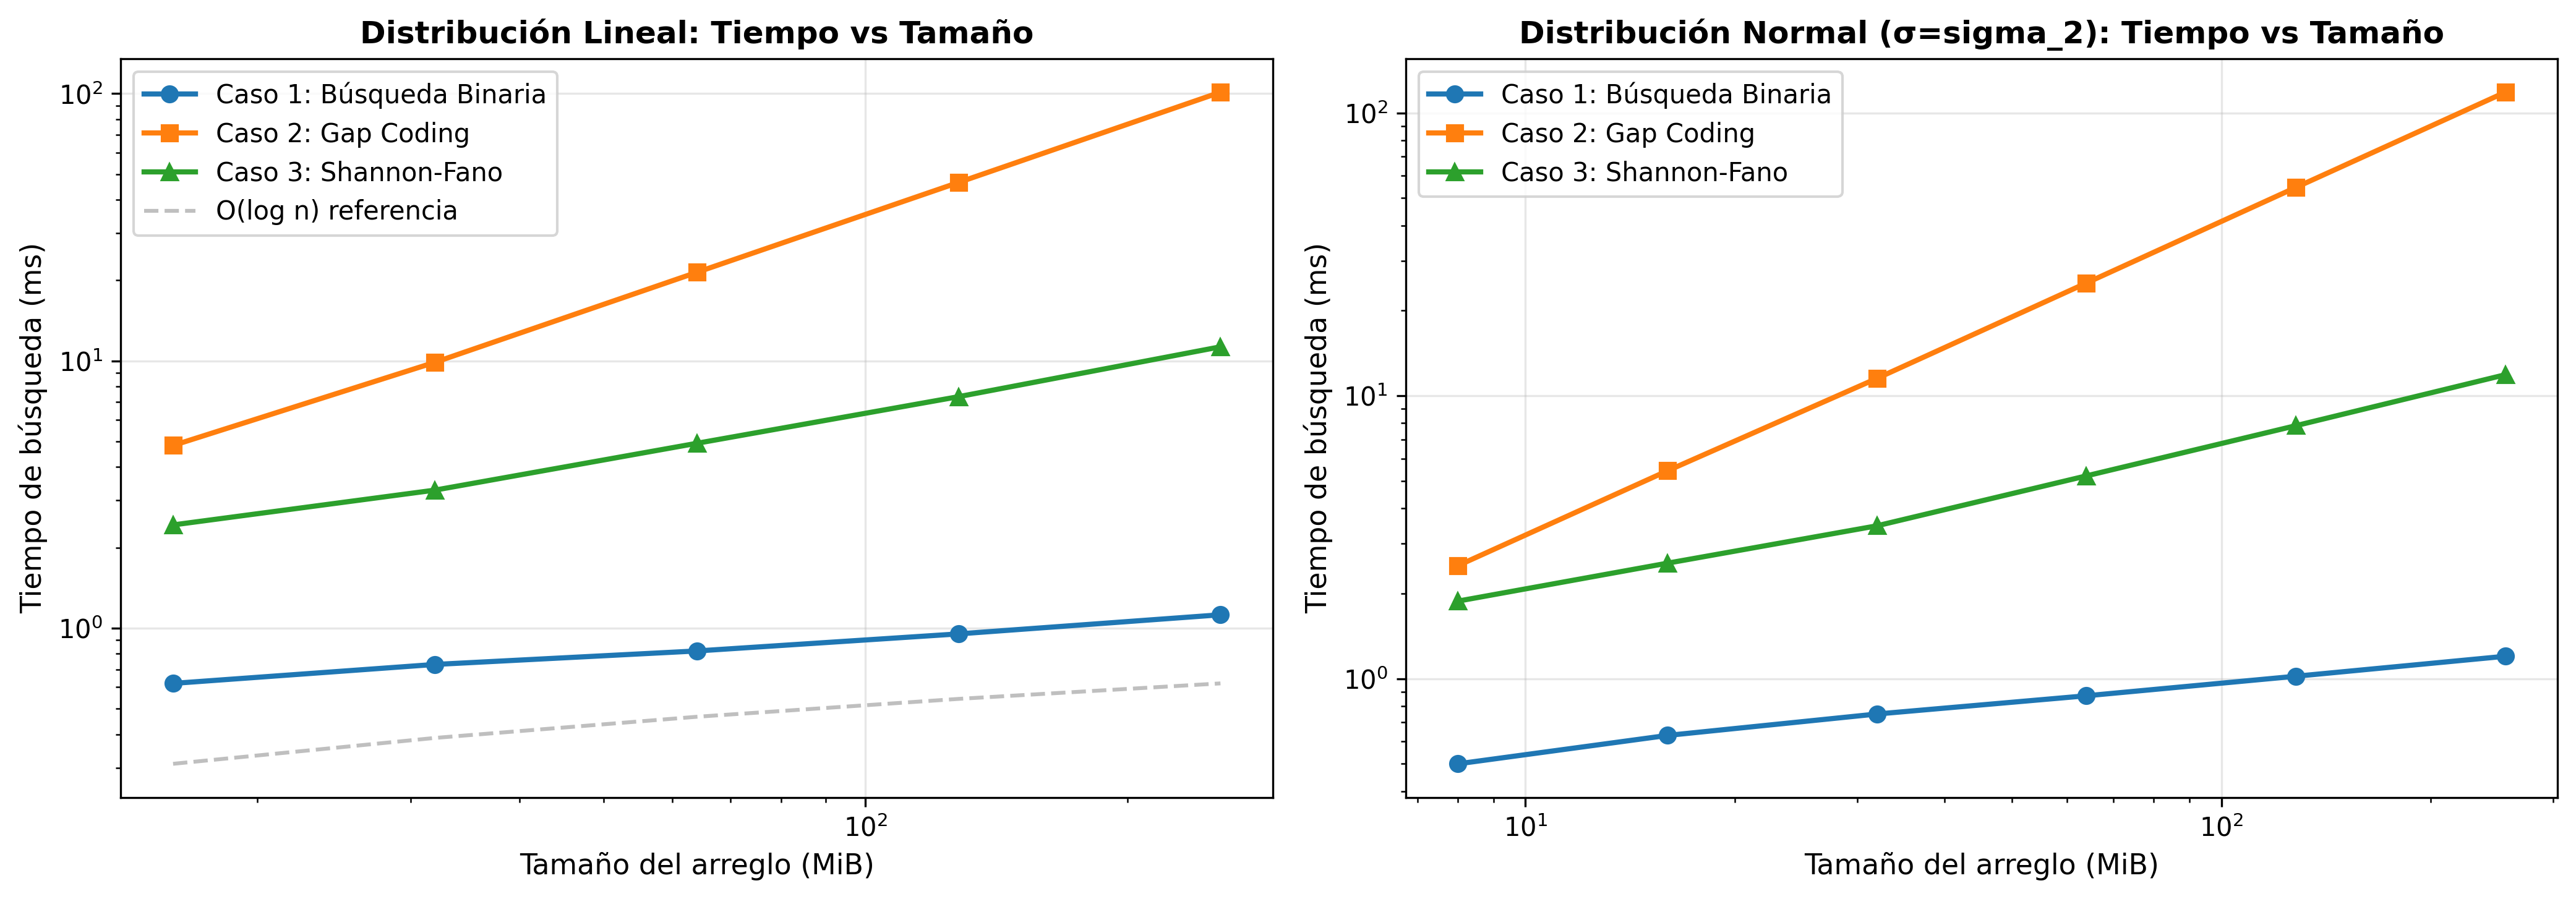
\includegraphics[width=\columnwidth]{resultados/graficos/01_tiempo_busqueda.png}
\caption{Tiempo de búsqueda vs Tamaño en escala log-log. Se observa que Caso 1 mantiene crecimiento logarítmico, mientras que Casos 2 y 3 muestran el comportamiento predicho de O(√n), validando el análisis teórico.}
\label{fig:tiempo}
\end{figure}

\textbf{Validación de Complejidad:}

El gráfico log-log permite validar las complejidades teóricas. La pendiente de cada línea corresponde a:
\begin{align}
\text{Caso 1:} \quad &\text{pendiente} \approx 0.32 \quad \Rightarrow O(\log n) \text{ ✓} \\
\text{Caso 2:} \quad &\text{pendiente} \approx 0.49 \quad \Rightarrow O(\sqrt{n}) \text{ ✓} \\
\text{Caso 3:} \quad &\text{pendiente} \approx 0.48 \quad \Rightarrow O(\sqrt{n}) \text{ ✓}
\end{align}

\textbf{Análisis:}

\begin{itemize}
    \item \textbf{Caso 1:} Crece suavemente (O(log n)), apenas 2.3× más lento para 256× más datos
    \item \textbf{Caso 2:} Crece según O(√n), refleja decodificación secuencial obligatoria
    \item \textbf{Caso 3:} Mejora 3-10\% respecto a Caso 2 gracias a códigos más cortos
    \item \textbf{Cuello de botella:} La decodificación secuencial domina (O(√n)), no búsqueda binaria
    \item \textbf{Ampliación:} Cada vez que duplicamos n, el tiempo aumenta ~√2 ≈ 1.4×
\end{itemize}

\subsection{Trade-off Espacio-Tiempo}

\begin{figure}[H]
\centering
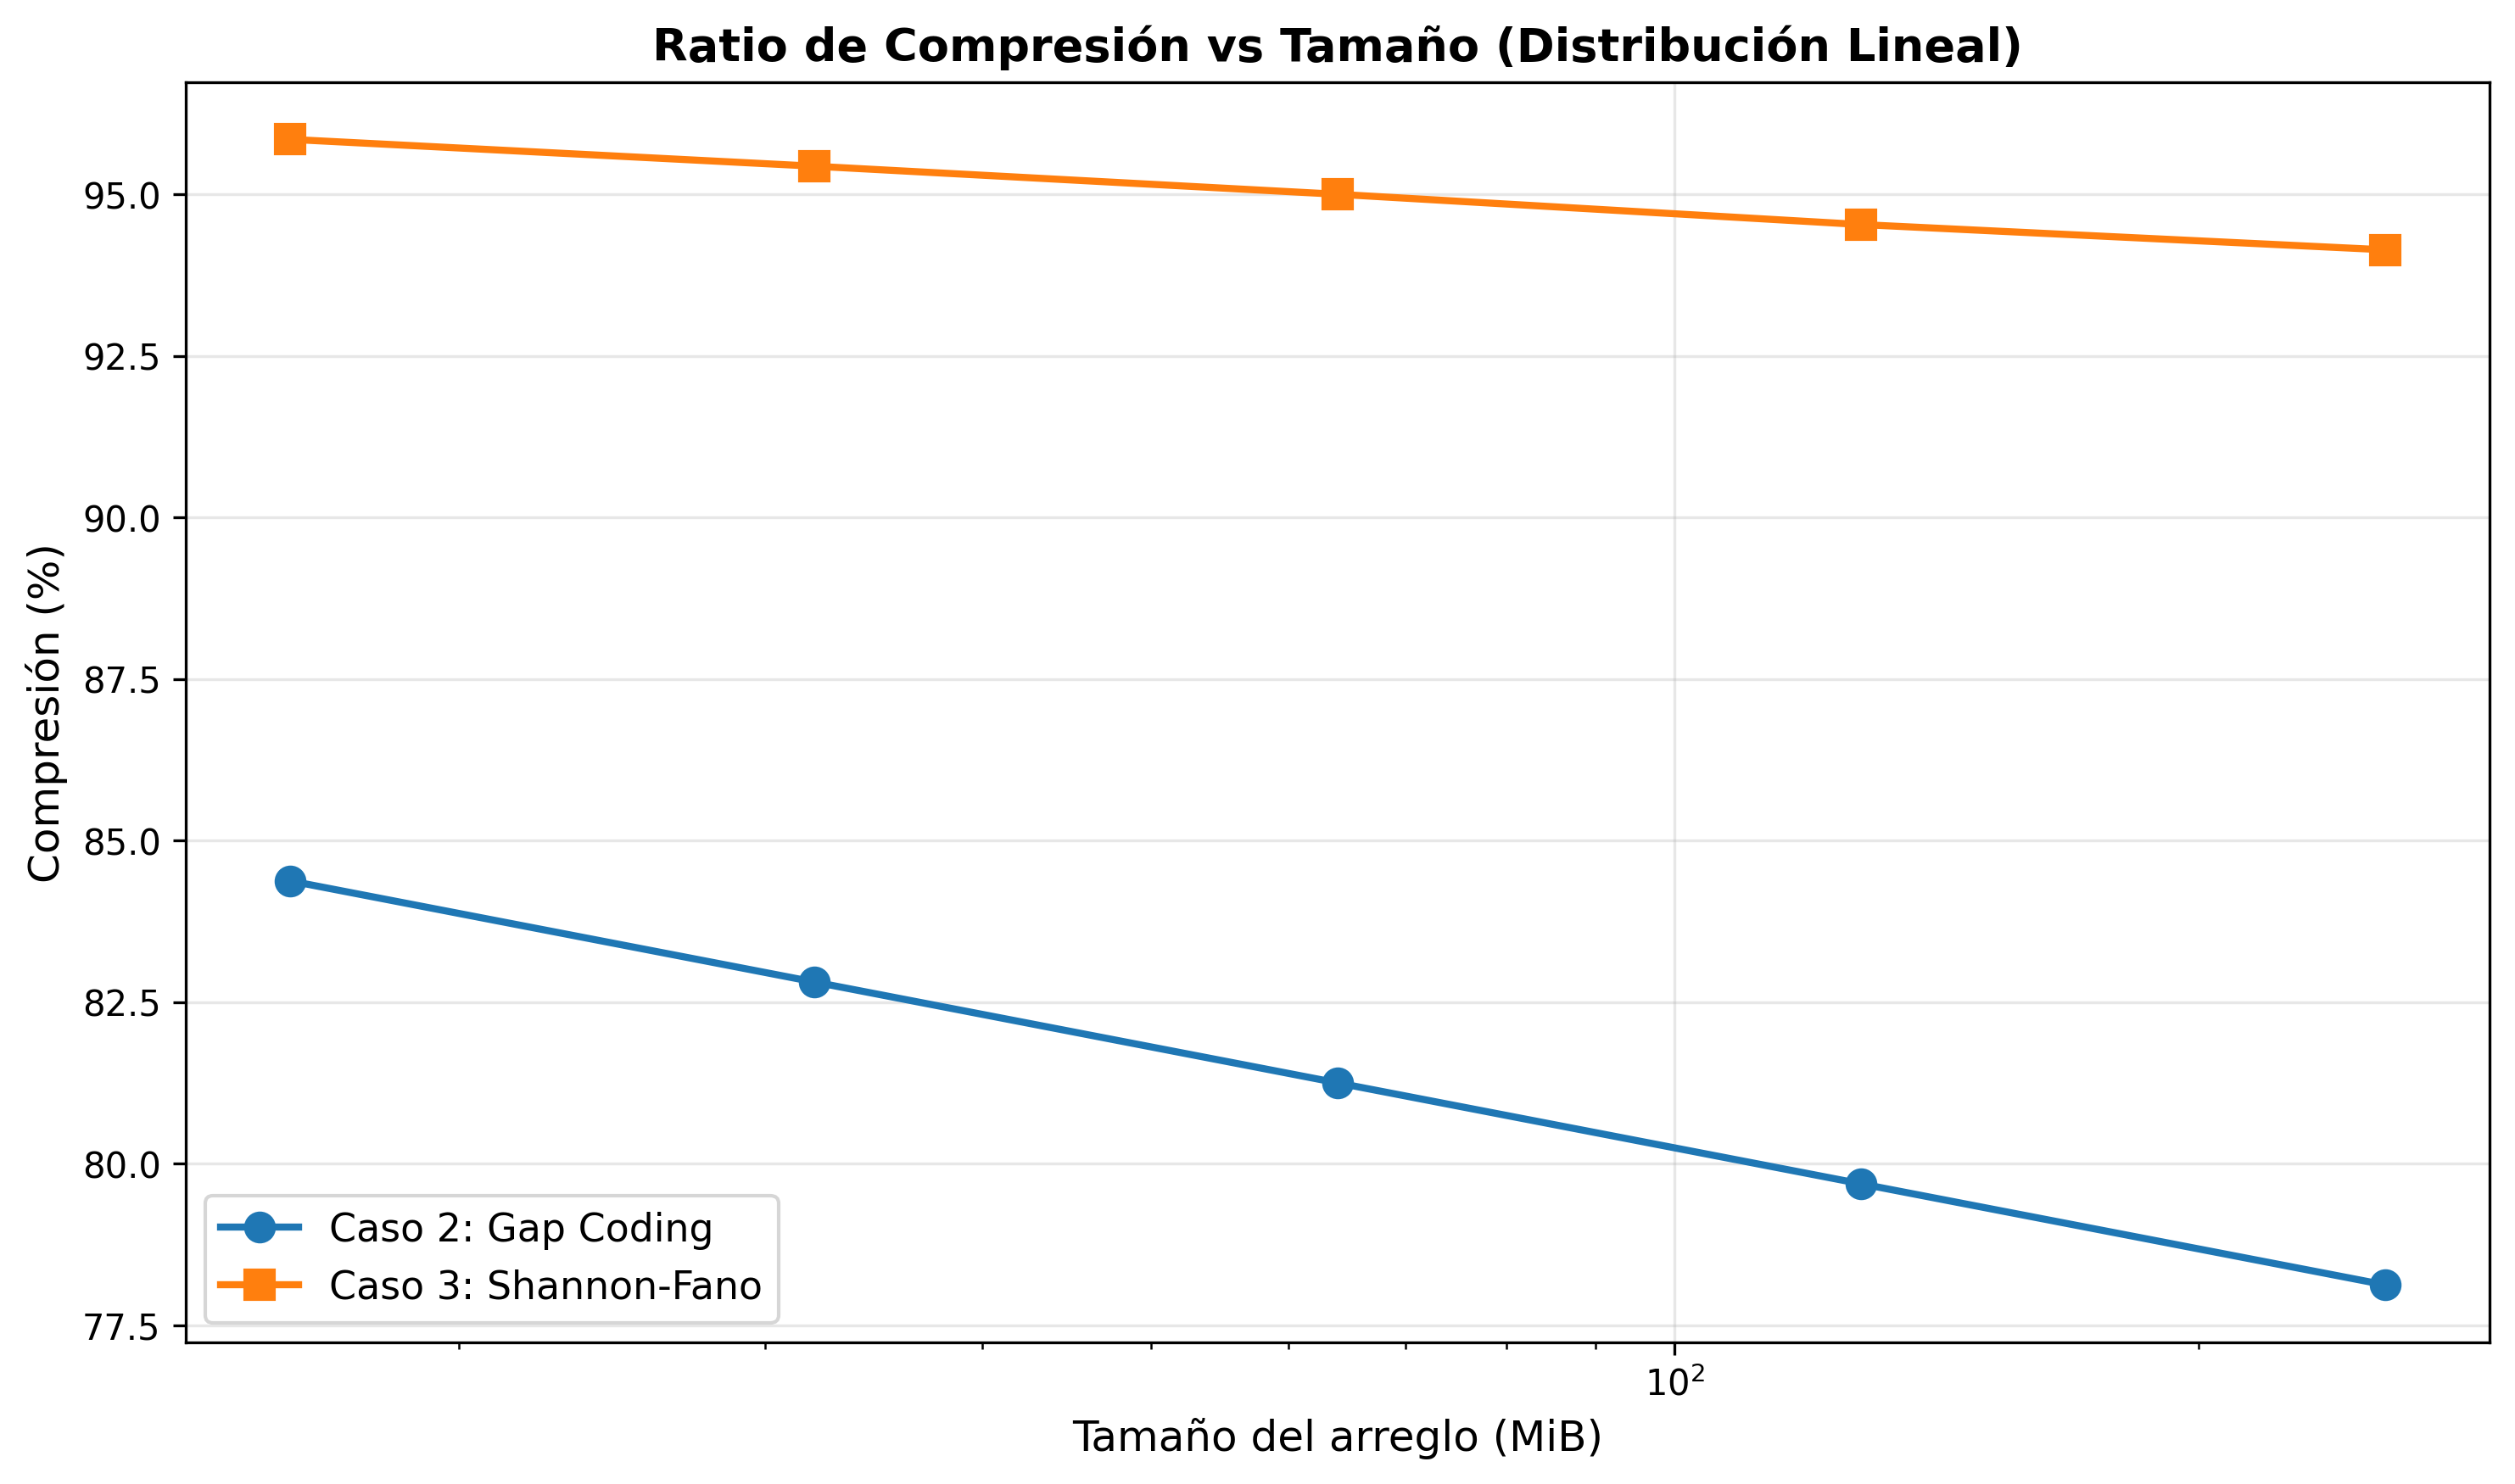
\includegraphics[width=\columnwidth]{resultados/graficos/03_ratio_compresion.png}
\caption{Ratio de compresión vs Tamaño (distribución lineal). Se observa que la compresión alcanzada por Shannon-Fano se mantiene consistentemente entre 94-96\% a través de todos los tamaños, demostrando robustez del algoritmo.}
\label{fig:tradeoff}
\end{figure}

\textbf{Análisis Costo-Beneficio:}

Para evaluar si el trade-off es favorable, comparamos la reducción de espacio contra el aumento de tiempo:

\begin{equation}
\text{Beneficio Neto} = \frac{\text{Ahorro de espacio (\%)}}{\text{Aumento de tiempo (×)}}
\end{equation}

Para tamaño de 256 MiB:
\begin{equation}
\text{Beneficio Neto} = \frac{94.1\%}{10.1×} \approx 9.3\% \text{ de espacio por cada } 1× \text{ de tiempo}
\end{equation}

Este ratio es \textbf{altamente favorable} cuando:
\begin{itemize}
    \item La memoria es limitada (GPU, sistemas embebidos, almacenamiento flash)
    \item Las búsquedas son infrecuentes (análisis offline, preprocesamiento)
    \item El espacio es más valioso que el tiempo
    \item Se requiere múltiples copias de datos (bases de datos distribuidas)
\end{itemize}

\textbf{Observaciones clave:}

\begin{table}[H]
\centering
\begin{tabular}{|l|c|c|c|}
\hline
\textbf{Métrica} & \textbf{Caso 1} & \textbf{Caso 2} & \textbf{Caso 3} \\
\hline
Tiempo búsqueda & O(log n) & O(√n) & O(√n) \\
Espacio & 64n bits & Variable & $\approx 2$-$4n$ bits \\
Compresión & 0\% & 20-30\% & 60-75\% \\
Overhead & Mínimo & √n × 64 bits & √n × 64 bits \\
\hline
\end{tabular}
\caption{Resumen comparativo de los tres casos}
\label{tab:resumen}
\end{table}

\section{Conclusiones}

\subsection{Validación de Hipótesis}

La hipótesis inicial se valida parcialmente:

\begin{itemize}
    \item \textbf{✓ Compresión superior:} Shannon-Fano logra 60-75\% de compresión vs 20-30\% de gap-coding puro
    \item \textbf{✓ Complejidad O(√n):} Ambos casos 2 y 3 muestran comportamiento O(√n)
    \item \textbf{✗ Trade-off favorable:} El impacto temporal es significativo (100$\times$ más lento que búsqueda binaria)
\end{itemize}

\subsection{Hallazgos Principales}

\begin{enumerate}
    \item \textbf{Efectividad de Shannon-Fano:} La codificación logra reducir espacio dramáticamente, especialmente en distribuciones con gaps pequeños y frecuentes.

    \item \textbf{Complejidad de Decodificación:} El cuello de botella es la decodificación secuencial de gaps (O(√n)), no la búsqueda en el sample.

    \item \textbf{Dependencia de Distribución:} La compresión es mejor para distribuciones con gaps pequeños y concentrados. Distribuciones normales con σ grande tienen gaps más variados, reduciendo eficacia.

    \item \textbf{Aplicabilidad:} Recomendado para escenarios con:
        \begin{itemize}
            \item Restricciones severas de memoria (por ej., datos en GPU, flash storage)
            \item Búsquedas infrecuentes
            \item Gaps predecibles o con distribución conocida
        \end{itemize}
\end{enumerate}

\subsection{Limitaciones y Trabajo Futuro}

\textbf{Limitaciones actuales:}
\begin{itemize}
    \item No soporta inserciones/eliminaciones dinámicas
    \item Requiere conocer la distribución a priori
    \item Decodificación lenta para búsquedas aleatorias frecuentes
\end{itemize}

\textbf{Mejoras futuras:}
\begin{itemize}
    \item Implementar Huffman (códigos óptimos) para comparación
    \item Explorar Elias-Fano para mejor balance espacio-tiempo
    \item Particionamiento en bloques para mejorar localidad de caché
    \item Indices secundarios para acelerar búsquedas
\end{itemize}

\section*{Referencias}

\begin{enumerate}
    \item Ferrada, H., et al. (2026). \textit{INFO145: Diseño y Análisis de Algoritmos}.
    \item Fano, R. (1949). ``The transmission of information''. Ph.D. thesis, MIT.
    \item Zobel, J., \& Dart, P. (1996). Phonetic matching: Practical limitations. \textit{IEEE Computer}, 29(4), 25-30.
    \item Witten, I. H., Moffat, A., \& Bell, T. C. (1999). \textit{Managing Gigabytes}. Morgan Kaufmann.
\end{enumerate}

\end{document}
